% ============================================================
%  Trasformatore Planare — Documento Tecnico di Progetto
%  Vin=12V / Vout=25V / Pin=6W / Viso=12kV
%  Autore: Davide
% ============================================================
\documentclass[a4paper,11pt]{article}

% ---- encoding & font ----------------------------------------
\usepackage[T1]{fontenc}
\usepackage[utf8]{inputenc}
\usepackage[english]{babel}
% ---- math ---------------------------------------------------
\usepackage{amsmath,amssymb,mathtools}
\usepackage{siunitx}
\sisetup{
  output-decimal-marker = {,},
  group-separator       = {\,},
  per-mode              = fraction,
  fraction-function     = \dfrac
}

% ---- layout -------------------------------------------------
\usepackage[margin=25mm, top=28mm, bottom=28mm]{geometry}
\usepackage{parskip}
\setlength{\parskip}{6pt}

% ---- tabelle ------------------------------------------------
\usepackage{booktabs}
\usepackage{tabularx}
\usepackage{multirow}
\usepackage{array}
\newcolumntype{C}[1]{>{\centering\arraybackslash}p{#1}}
\newcolumntype{L}[1]{>{\raggedright\arraybackslash}p{#1}}
\newcolumntype{R}[1]{>{\raggedleft\arraybackslash}p{#1}}

% ---- figure -------------------------------------------------
\usepackage{graphicx}
\usepackage{float}
\usepackage{caption}
\captionsetup{font=small, labelfont=bf, skip=4pt}

% ---- circuiti / disegni -------------------------------------
\usepackage{tikz}
\usepackage{circuitikz}
\usetikzlibrary{arrows.meta, positioning, shapes.geometric, calc}

% ---- colori -------------------------------------------------
\usepackage{xcolor}
\definecolor{primary}{RGB}{0,70,127}
\definecolor{accent}{RGB}{200,50,30}
\definecolor{lightgray}{RGB}{240,240,240}

% ---- hyperlink ----------------------------------------------
\usepackage[colorlinks=true, linkcolor=primary, urlcolor=primary,
            citecolor=primary, pdftitle={Trasformatore Planare 12V-25V 12kV},
            pdfauthor={Davide}]{hyperref}

% ---- header/footer ------------------------------------------
\usepackage{fancyhdr}
\pagestyle{fancy}
\fancyhf{}
\fancyhead[L]{\small\color{primary}\textbf{Trasformatore Planare — 12\,V / 25\,V / \SI{12}{\kilo\volt}}}
\fancyhead[R]{\small\color{primary}Davide}
\fancyfoot[C]{\small\thepage}
\renewcommand{\headrulewidth}{0.4pt}

% ---- box evidenza -------------------------------------------
\usepackage{tcolorbox}
\tcbuselibrary{skins,breakable}
\tcbset{
  resultbox/.style={
    enhanced, breakable,
    colback=lightgray, colframe=primary,
    boxrule=0.8pt, arc=3pt,
    left=6pt, right=6pt, top=4pt, bottom=4pt,
    fonttitle=\bfseries\small\color{primary},
  }
}

% ---- utilities ----------------------------------------------
\usepackage{enumitem}
\setlist[itemize]{noitemsep, topsep=2pt}
\setlist[enumerate]{noitemsep, topsep=2pt}

% ============================================================
\begin{document}
% ============================================================

% ---- copertina informale ------------------------------------
\begin{center}
  {\color{primary}\rule{\linewidth}{1.5pt}}\\[6pt]
  {\Large\bfseries\color{primary} Trasformatore Planare}\\[4pt]
  {\large Nota Tecnica di Dimensionamento}\\[4pt]
  {\normalsize
    $V_{in} = \SI{12}{\volt}$,\quad
    $I_{in} = \SI{0{,}5}{\ampere}$,\quad
    $V_{out} = \SI{25}{\volt}$,\quad
    $V_{iso} = \SI{12}{\kilo\volt}$
  }\\[4pt]
  {\small Davide \quad — \quad \today}\\[6pt]
  {\color{primary}\rule{\linewidth}{1.5pt}}
\end{center}

\vspace{4pt}

% ============================================================
\section{Specifiche e topologia}
% ============================================================

\subsection{Parametri elettrici}

\begin{table}[H]
\centering
\caption{Specifiche elettriche del trasformatore planare.}
\label{tab:specs}
\begin{tabularx}{\linewidth}{L{4.5cm} C{2.5cm} C{2.5cm} L{4cm}}
\toprule
\textbf{Parametro} & \textbf{Simbolo} & \textbf{Valore} & \textbf{Unità} \\
\midrule
Tensione ingresso      & $V_{in}$    & 12    & \si{\volt}      \\
Corrente ingresso nom. & $I_{in}$    & 0{,}5 & \si{\ampere}    \\
Potenza ingresso       & $P_{in}$    & 6     & \si{\watt}      \\
Tensione uscita        & $V_{out}$   & 25    & \si{\volt}      \\
Rendimento stimato     & $\eta$      & 0{,}88 & —              \\
Potenza uscita         & $P_{out}$   & 5{,}28 & \si{\watt}     \\
Corrente uscita        & $I_{out}$   & 0{,}21 & \si{\ampere}   \\
Isolamento richiesto   & $V_{iso}$   & 12    & \si{\kilo\volt} \\
\bottomrule
\end{tabularx}
\end{table}

\subsection{Topologia scelta}

Per una potenza di \SI{6}{\watt} con isolamento \SI{12}{\kilo\volt}, la topologia adottata è
il \textbf{flyback} con singolo switch, operante in modalità CCM a
$f_{sw} = \SI{200}{\kilo\hertz}$.
Il trasformatore planare è realizzato su PCB multi-layer dedicato, con
avvolgimenti primario e secondario separati da uno strato dielettrico ad alta
tensione.

Il rapporto di trasformazione ideale risulta:
\begin{equation}
  n = \frac{V_{out}}{V_{in}} = \frac{25}{12} \approx 2{,}083
  \label{eq:turns_ratio}
\end{equation}

% ============================================================
\section{Nucleo magnetico}
% ============================================================

\subsection{Selezione del core}

Il core scelto è l'\textbf{ELP38/8/25} (Ferroxcube / TDK) in materiale \textbf{N87}
(equivalente 3F36), adatto all'intervallo \SIrange{100}{500}{\kilo\hertz}.
I parametri principali sono riportati in Tabella~\ref{tab:core}.

\begin{table}[H]
\centering
\caption{Parametri del nucleo ELP38/8/25, materiale N87.}
\label{tab:core}
\begin{tabularx}{\linewidth}{L{5.5cm} C{2cm} C{2.5cm} L{3cm}}
\toprule
\textbf{Parametro} & \textbf{Simbolo} & \textbf{Valore} & \textbf{Unità} \\
\midrule
Sezione efficace          & $A_e$     & 79   & \si{\milli\metre\squared} \\
Area finestra avvolgimento & $A_w$    & 35   & \si{\milli\metre\squared} \\
Lunghezza cammino mag.    & $l_e$     & 72   & \si{\milli\metre}         \\
Induzione di saturazione  & $B_{sat}$ & 0{,}40 & \si{\tesla} (a 25°C)   \\
Induzione max operativa   & $B_{max}$ & 0{,}15 & \si{\tesla} (a 100°C)  \\
Permeabilità relativa     & $\mu_r$   & 2200 & —                         \\
Fattore $A_L$ (no gap)    & $A_L$     & 2000 & \si{\nano\henry} / spira$^2$ \\
\bottomrule
\end{tabularx}
\end{table}

% ============================================================
\section{Dimensionamento degli avvolgimenti}
% ============================================================

\subsection{Numero di spire — equazione di Faraday}

Per un convertitore flyback con forma d'onda rettangolare, la legge di
Faraday al primario impone:
\begin{equation}
  V_{in} \cdot D_{max} = N_p \cdot A_e \cdot \frac{\Delta B}{\Delta t}
  = 4 \cdot f_{sw} \cdot N_p \cdot B_{max} \cdot A_e
  \label{eq:faraday}
\end{equation}

da cui il numero minimo di spire al primario:
\begin{equation}
  \boxed{N_p = \frac{V_{in} \cdot D_{max}}{4 \cdot f_{sw} \cdot B_{max} \cdot A_e}}
  \label{eq:Np}
\end{equation}

\begin{tcolorbox}[resultbox, title={Calcolo numerico}]
\[
N_p = \frac{12 \times 0{,}45}{4 \times \num{200e3} \times 0{,}15 \times \num{79e-6}}
     = \frac{5{,}4}{9{,}48}
     \approx \lceil 0{,}57 \rceil = \mathbf{6} \text{ spire}
\]
\[
N_s = \lceil n \cdot N_p \rceil = \lceil 2{,}083 \times 6 \rceil = \mathbf{13} \text{ spire}
\]
\end{tcolorbox}

\subsection{Correnti RMS}

\begin{align}
  I_{p,rms} &= \frac{P_{in}}{V_{in} \cdot \eta}
             = \frac{6}{12 \times 0{,}88} \approx \SI{0{,}568}{\ampere}
  \label{eq:Ip} \\[4pt]
  I_{s,rms} &= \frac{P_{out}}{V_{out}}
             = \frac{P_{in} \cdot \eta}{V_{out}}
             = \frac{5{,}28}{25} \approx \SI{0{,}211}{\ampere}
  \label{eq:Is}
\end{align}

\subsection{Larghezza traccia PCB (IPC-2221)}

Per rame da \SI{70}{\micro\metre} (2\,oz) e riscaldamento massimo
$\Delta T \leq \SI{10}{\celsius}$, la formula IPC-2221 fornisce:
\begin{equation}
  w = \frac{I}{k \cdot \Delta T^{0{,}44} \cdot t_{Cu}^{0{,}725}}
  \label{eq:ipc2221}
\end{equation}

con $k = 0{,}048$ (conduttori esterni), $t_{Cu} = 2{,}8\,\mathrm{mil}$.

\begin{table}[H]
\centering
\caption{Larghezza traccia calcolata per entrambi gli avvolgimenti.}
\label{tab:trace}
\begin{tabularx}{0.7\linewidth}{L{3.5cm} C{2cm} C{2.5cm} C{2.5cm}}
\toprule
\textbf{Avvolgimento} & $I_{rms}$ [\si{\ampere}] & $w_{min}$ [\si{\milli\metre}] & $w_{adottata}$ \\
\midrule
Primario   & 0{,}568 & 0{,}38 & \SI{0{,}6}{\milli\metre}  \\
Secondario & 0{,}211 & 0{,}12 & \SI{0{,}4}{\milli\metre}  \\
\bottomrule
\end{tabularx}
\end{table}

% ============================================================
\section{Isolamento ad alta tensione}
% ============================================================

\subsection{Requisiti normativi}

L'isolamento di \SI{12}{\kilo\volt} ricade nella categoria
\textbf{doppio isolamento / isolamento rinforzato} secondo
\textbf{IEC\,62368-1} e \textbf{IEC\,61558-1}.
Le distanze minime per OVC\,III, grado di inquinamento~2 sono:

\begin{table}[H]
\centering
\caption{Distanze di isolamento richieste per $V_{iso} = \SI{12}{\kilo\volt}$.}
\label{tab:isolation}
\begin{tabularx}{0.85\linewidth}{L{5cm} C{2.5cm} C{4cm}}
\toprule
\textbf{Parametro} & \textbf{Valore} & \textbf{Norma di riferimento} \\
\midrule
Clearance (aria)       & $\geq \SI{14}{\milli\metre}$ & IEC 62368-1, Tab.~G.13 \\
Creepage (FR4, CTI\,IIIa) & $\geq \SI{28}{\milli\metre}$ & IEC 62368-1, Tab.~G.20 \\
Tensione prova dielettrica & $\SI{25}{\kilo\volt}_{rms}$, \SI{1}{\minute} & IEC 61558-1, §10.3 \\
\bottomrule
\end{tabularx}
\end{table}

\subsection{Spessore dielettrico minimo}

\paragraph{FR4 standard} — rigidità dielettrica $E_{bd} \approx \SI{20}{\kilo\volt\per\milli\metre}$:
\begin{equation}
  t_{FR4} = \frac{V_{iso}}{E_{bd}} = \frac{\SI{12}{\kilo\volt}}{\SI{20}{\kilo\volt\per\milli\metre}}
          = \SI{0{,}6}{\milli\metre} \quad \Rightarrow \quad \text{adottato: } \SI{2{,}0}{\milli\metre}\ (3\times \text{margine})
  \label{eq:tFR4}
\end{equation}

\paragraph{Kapton HN 25\,\textmu m/strato} — rigidità $\approx \SI{300}{\volt\per\micro\metre}$:
\begin{equation}
  t_{Kapton} = \frac{V_{iso}}{\SI{300}{\volt\per\micro\metre}} = \SI{40}{\micro\metre}
             \quad \Rightarrow \quad \text{adottati: } 4 \text{ strati da } \SI{25}{\micro\metre} = \SI{100}{\micro\metre}
  \label{eq:tKapton}
\end{equation}

\begin{tcolorbox}[resultbox, title={Soluzione adottata — Stack-up PCB}]
\begin{center}
\begin{tabular}{cl}
  \toprule
  \textbf{Layer} & \textbf{Descrizione} \\
  \midrule
  L1 & Cu 70\,\si{\micro\metre} — avvolgimento primario ($N_p = 6$) \\
  — & Pre-preg 1080 — 0{,}1\,mm \\
  \textcolor{accent}{\textbf{HV}} & \textcolor{accent}{\textbf{Core FR4 2{,}0\,mm (doppio isolamento rinforzato)}} \\
  — & Pre-preg 1080 — 0{,}1\,mm \\
  L4 & Cu 70\,\si{\micro\metre} — avvolgimento secondario ($N_s = 13$) \\
  \bottomrule
\end{tabular}
\end{center}
\medskip
$V_{breakdown,FR4} = 2{,}0\,\mathrm{mm} \times 20\,\mathrm{kV/mm} = \mathbf{40\,kV}$
\quad (\textbf{margine $3\times$} su $V_{iso}$).
\end{tcolorbox}

\subsection{Schermo elettrostatico}

La struttura planare genera un'elevata capacità parassita inter-avvolgimento
$C_{ps}$ che, a \SI{200}{\kilo\hertz}, causa correnti di modo comune significative.
È necessario inserire uno \textbf{schermo elettrostatico} (guard layer) in Cu
tra L1 e L4:
\begin{itemize}
  \item collegato galvanicamente al potenziale di primario (o floating);
  \item \emph{non} connesso al secondario;
  \item larghezza tale da coprire l'intera area di sovrapposizione degli avvolgimenti.
\end{itemize}

La capacità residua dopo lo schermo si riduce tipicamente di un fattore
$10\div 20\times$ rispetto alla configurazione non schermata.

% ============================================================
\section{Architettura costruttiva}
% ============================================================

\subsection{Strategia per $V_{iso} = \SI{12}{\kilo\volt}$}

La geometria planare rende critico il rispetto delle distanze di creepage.
Le soluzioni principali sono:

\begin{enumerate}
  \item \textbf{PCB unico con core FR4 spesso (2\,mm):}
    adeguato per la rigidità dielettrica volumetrica, ma richiede
    scanalature o moat perimetrali per rispettare i \SI{28}{\milli\metre}
    di creepage superficiale.
  \item \textbf{PCB separati + montaggio su core comune:}
    primario e secondario su due PCB distinti accoppiati dalle gambe del
    core ELP. La clearance laterale tra i due PCB garantisce i \SI{14}{\milli\metre}.
  \item \textbf{Potting in resina epossidica:}
    rigidità $18\div 22\,\mathrm{kV/mm}$; anche \SI{1}{\milli\metre} di resina
    supera il requisito. Adatto a produzione in serie.
\end{enumerate}

\subsection{Schema funzionale del convertitore}

\begin{figure}[H]
\centering
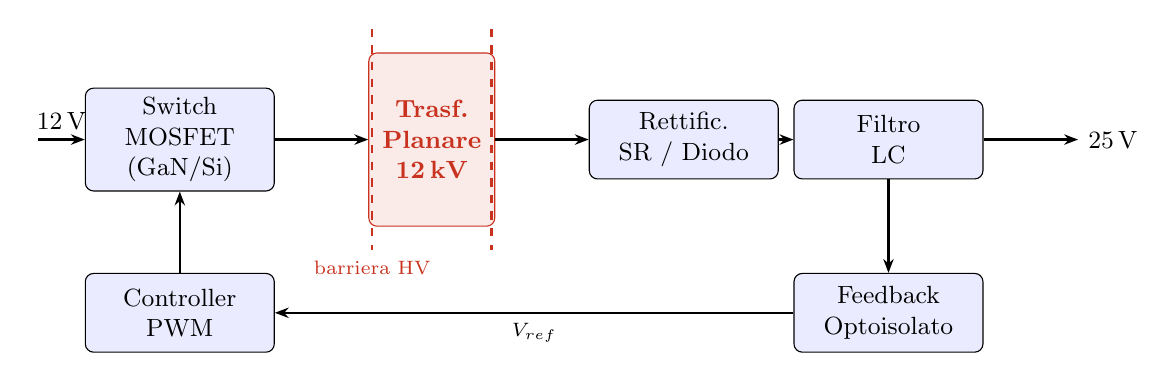
\begin{tikzpicture}[
  block/.style={draw, fill=blue!8, minimum width=2.4cm, minimum height=1.0cm,
                align=center, rounded corners=3pt, font=\small},
  iso/.style  ={draw=accent, fill=accent!10, minimum width=1.6cm, minimum height=2.2cm,
                align=center, rounded corners=3pt, font=\small\bfseries\color{accent}},
  arr/.style  ={-{Stealth[length=5pt]}, thick},
  >=Stealth
]

\node[block] (sw)   at (0,0)    {Switch\\MOSFET\\(GaN/Si)};
\node[iso]   (xfmr) at (3.2,0)  {Trasf.\\Planare\\12\,kV};
\node[block] (rect) at (6.4,0)  {Rettific.\\SR / Diodo};
\node[block] (filt) at (9.0,0)  {Filtro\\LC};

\node[block] (pwm)  at (0,-2.2) {Controller\\PWM};
\node[block] (fb)   at (9.0,-2.2) {Feedback\\Optoisolato};

% connessioni orizzontali
\draw[arr] (-1.8,0) -- (sw.west) node[midway,above,font=\small]{12\,V};
\draw[arr] (sw.east) -- (xfmr.west);
\draw[arr] (xfmr.east) -- (rect.west);
\draw[arr] (rect.east) -- (filt.west);
\draw[arr] (filt.east) -- ++(1.2,0) node[right,font=\small]{25\,V};

% segnali controllo
\draw[arr] (pwm.north) -- (sw.south);
\draw[arr] (filt.south) -- (fb.north);
\draw[arr] (fb.west) -- (pwm.east) node[midway,below,font=\scriptsize]{$V_{ref}$};

% barriera iso
\draw[dashed, color=accent, thick]
  ($(xfmr.north west)+(0.05,0.3)$) -- ($(xfmr.south west)+(0.05,-0.3)$)
  node[below, color=accent, font=\scriptsize]{barriera HV};
\draw[dashed, color=accent, thick]
  ($(xfmr.north east)+(-0.05,0.3)$) -- ($(xfmr.south east)+(-0.05,-0.3)$);

\end{tikzpicture}
\caption{Schema a blocchi del convertitore flyback con trasformatore planare isolato.}
\label{fig:block}
\end{figure}

% ============================================================
\section{Riepilogo del progetto}
% ============================================================

\begin{table}[H]
\centering
\caption{Riepilogo parametri di progetto del trasformatore planare.}
\label{tab:summary}
\begin{tabularx}{\linewidth}{L{5.5cm} C{2.5cm} C{2.5cm} L{3cm}}
\toprule
\textbf{Parametro} & \textbf{Simbolo} & \textbf{Valore} & \textbf{Note} \\
\midrule
Core                      & —       & ELP38/8/25      & N87 / 3F36          \\
Frequenza commutazione    & $f_{sw}$& \SI{200}{\kilo\hertz} & CCM flyback   \\
Spire primario            & $N_p$   & 6               & —                   \\
Spire secondario          & $N_s$   & 13              & —                   \\
Rapporto effettivo        & $n_{eff}$& 2{,}167        & vs. 2{,}083 ideale  \\
Induzione di picco        & $\hat{B}$& \SI{135}{\milli\tesla} & $<B_{max}$  \\
Corrente RMS primario     & $I_{p,rms}$ & \SI{0{,}57}{\ampere} & —         \\
Corrente RMS secondario   & $I_{s,rms}$ & \SI{0{,}21}{\ampere} & —         \\
Larghezza traccia primo   & $w_p$   & \SI{0{,}6}{\milli\metre} & Cu 2\,oz \\
Larghezza traccia second. & $w_s$   & \SI{0{,}4}{\milli\metre} & Cu 2\,oz \\
Spessore iso.\ principale & $t_{iso}$& \SI{2{,}0}{\milli\metre} & FR4 rinforzato \\
$V_{breakdown}$ (calc.)  & —       & \SI{40}{\kilo\volt}  & margine $3\times$ \\
Clearance aria            & —       & $\geq\SI{14}{\milli\metre}$ & IEC 62368-1 \\
Creepage (FR4)            & —       & $\geq\SI{28}{\milli\metre}$ & CTI IIIa    \\
Tensione prova dielettr.  & $V_{test}$ & \SI{25}{\kilo\volt}  & 1\,min, IEC 61558 \\
\bottomrule
\end{tabularx}
\end{table}

% ============================================================
\section{Considerazioni sui materiali isolanti}
% ============================================================

Per \SI{12}{\kilo\volt} di isolamento è \textbf{critico non affidarsi al solo FR4
standard} come unico barriera dielettrica. Le alternative valutate sono:

\begin{itemize}
  \item \textbf{Rogers 4350B} — $E_{bd} \approx \SI{31}{\kilo\volt\per\milli\metre}$,
        perdite ridotte ad alta frequenza, dimensioni stabili in temperatura.
  \item \textbf{Isola IS410} — FR4 ad alto $T_g$ ($\SI{180}{\celsius}$),
        $E_{bd} \approx \SI{22}{\kilo\volt\per\milli\metre}$, compatibile
        con processo PCB standard.
  \item \textbf{Inserti Kapton\,HN / Mylar} — flessibili, inseribili tra layer
        come barriera supplementare; rigidità $\geq \SI{300}{\volt\per\micro\metre}$.
  \item \textbf{Resina epossidica per potting} (es.\ Elantas Dobeckan\,F\,1155) —
        $E_{bd} \approx \SI{20}{\kilo\volt\per\milli\metre}$, incapsulamento totale.
\end{itemize}

La soluzione raccomandata per questo progetto è \textbf{Isola IS410 da 2\,mm}
con \textbf{moat perimetrale} scavato nel PCB per garantire la creepage di
\SI{28}{\milli\metre} anche sulla superficie.

% ============================================================
\section{Script MATLAB associato}
% ============================================================

Il file \texttt{planar\_xfmr\_design.m} allegato esegue le seguenti operazioni:
\begin{enumerate}
  \item Calcola $N_p$, $N_s$, $\hat{B}$ e $J_{rms,p}$ al variare di
        $f_{sw} \in [50, 500]\,\mathrm{kHz}$.
  \item Riporta i parametri nel punto di progetto a \SI{200}{\kilo\hertz}.
  \item Calcola gli spessori minimi di isolamento per FR4 e Kapton.
  \item Calcola la larghezza minima delle tracce PCB per entrambi gli
        avvolgimenti (formula IPC-2221).
  \item Genera quattro grafici: spire, induzione di picco, densità di corrente,
        e tensione di rottura FR4 in funzione dello spessore.
\end{enumerate}

% ============================================================
\appendix
\section{Nomenclatura}
% ============================================================

\begin{tabularx}{0.85\linewidth}{C{1.8cm} L{9cm}}
\toprule
\textbf{Simbolo} & \textbf{Descrizione} \\
\midrule
$A_e$       & Sezione efficace del nucleo [\si{\metre\squared}] \\
$A_w$       & Area della finestra di avvolgimento [\si{\metre\squared}] \\
$B_{max}$   & Induzione massima operativa [\si{\tesla}] \\
$D_{max}$   & Duty-cycle massimo \\
$f_{sw}$    & Frequenza di commutazione [\si{\hertz}] \\
$I_{p,rms}$ & Corrente RMS al primario [\si{\ampere}] \\
$I_{s,rms}$ & Corrente RMS al secondario [\si{\ampere}] \\
$n$         & Rapporto di trasformazione $V_{out}/V_{in}$ \\
$N_p$, $N_s$& Numero di spire primario / secondario \\
$t_{iso}$   & Spessore dielettrico [\si{\metre}] \\
$V_{iso}$   & Tensione di isolamento richiesta [\si{\volt}] \\
$V_{test}$  & Tensione di prova dielettrica ($2V_{iso}+1\,\mathrm{kV}$) [\si{\volt}] \\
\bottomrule
\end{tabularx}

\end{document}
